\documentclass[a4paper,10pt]{article}

\usepackage{graphicx}
\usepackage{natbib}
\usepackage{amsmath}
\usepackage{amssymb}
\usepackage{bm}
\usepackage{ulem}
\usepackage{enumerate}
\usepackage{siunitx}
% \usepackage{extarrows}
%\usepackage[cm]{fullpage}
\usepackage{hyperref}
%\usepackage[dvips,bookmarks=false,pdfstartview={XYZ null null 1.00},pdfstartpage=1]{hyperref}	%sets pdf viewing options
\usepackage{mathtools}	%needed for dcase environment, loads amsmath package
\usepackage{geometry}
\geometry{margin=0.7in}
%\topmargin -100pt
%
%\usepackage{tabularx,array,booktabs}
%\renewcommand{\tabularxcolumn}[1]{m{#1}}
%
\def\apj{ApJ}
\def\apss{Ap{\&}SS}
\def\mnras{MNRAS}
\def\aap{A\&A}
\def\apjl{ApJ}
\def\gafd{GAFD}
\def\jfm{JFM}
\def\physrep{PhR}
\def\pre{PhRvE}
\def\prl{PhRvL}
\def\apjs{ApJS}
\def\pasa{PASA}
\def\pasj{PASJ}
\def\nat{Nature}
\def\pasp{PASP}
\def\ssr{SSRv}
\def\araa{ARA\&A}
\def\aj{AJ}
\def\sgg{Stud.\ Geophys.\ Geod.}
\def\na{New\ Astron.}
\def\aapr{ARA\&A}
\def\gapfd{GApFD}
\def\an{AN}
%
\newcommand{\zhat}{\hat{z}}
\newcommand{\What}{\widehat{W}}
\newcommand{\Vhat}{\widehat{V}}
\newcommand{\Exp}[1]{{\rm e}^{#1}}
\newcommand{\Log}{\mathrm{Log}}
\newcommand{\del}{\partial}
\newcommand{\Del}{{\nabla}}
\newcommand{\bfDel}{\bm{\nabla}}
\newcommand{\bmDel}{\bm{\nabla}}
\newcommand{\bfomega}{\bm{\omega}}
\newcommand{\bmomega}{\bm{\omega}}
\newcommand{\alp}{\alpha}
\newcommand{\Gam}{\Gamma}
\newcommand{\eps}{\epsilon}
\newcommand{\Delsq}{\nabla^2}
\newcommand{\Emf}{\bm{\mathcal{E}}}
\newcommand{\Fmf}{\bm{F}}
\newcommand{\Flux}{\bm{\mathcal{F}}}
\newcommand{\Bs}{\mathcal{B}}
\newcommand{\Bsr}{\mathcal{B}_r}
\newcommand{\Bsp}{\mathcal{B}_\phi}
\newcommand{\Bsz}{\mathcal{B}_z}
\newcommand{\bfU}{\bm{U}}
\newcommand{\bfB}{\bm{B}}
\newcommand{\bfu}{\bm{u}}
\newcommand{\bfb}{\bm{b}}
\newcommand{\bmb}{\bm{b}}
\newcommand{\bfz}{\bm{z}}
\newcommand{\bmz}{\bm{z}}
\newcommand{\bfztilde}{\widetilde{\bm{z}}}
\newcommand{\bfj}{\bm{j}}
\newcommand{\bmj}{\bm{j}}
\newcommand{\Emfr}{\mathcal{E}_r}
\newcommand{\Emfp}{\mathcal{E}_\phi}
\newcommand{\Emfz}{\mathcal{E}_z}
\newcommand{\Fmfr}{F_r}
\newcommand{\Fmfp}{F_\phi}
\newcommand{\Fmfz}{F_z}
\newcommand{\Fluxr}{\mathcal{F}_r}
\newcommand{\Fluxphi}{\mathcal{F}_\phi}
\newcommand{\Fluxz}{\mathcal{F}_z}
\newcommand{\mean}[1]{\overline{#1}}
\newcommand{\meanv}[1]{\overline{\bm{#1}}}
\newcommand{\avg}[1]{\left<{#1}\right>}
\newcommand{\corr}{_\mathrm{c}}						%correlation
\newcommand{\corot}{_\mathrm{c}}						%corotation
\newcommand{\D}{_\mathrm{D}}						%disc
\newcommand{\eq}{_\mathrm{eq}}						%equipartition
\newcommand{\rms}{_\mathrm{0}}						%rms
\newcommand{\f}{_\mathrm{0}}					   	%forcing
\newcommand{\1}{_\mathrm{1}}					   	%forcing
\newcommand{\2}{_\mathrm{2}}					   	%forcing
\newcommand{\kin}{_\mathrm{k}}			   		%kinematic
\newcommand{\magn}{_\mathrm{m}}			   		%magnetic
\newcommand{\turb}{_\mathrm{t}}			   		%turbulent
\newcommand{\etat}{\eta_\mathrm{t}}			   	%turbulent diffusivity
\newcommand{\Turb}{\mathrm{t}}			   		%turbulent, in-line
\newcommand{\crit}{_\mathrm{c}}			   		%critical
\newcommand{\dip}{_\mathrm{d}}			   		%dipole
\newcommand{\sat}{_\mathrm{sat}}			   	%saturated
\newcommand{\const}{\mathrm{const}}			   	%constant
\newcommand{\mx}{\mathrm{max}}			   		%maximum
\newcommand{\ma}{_\mathrm{max}}			   		%maximum
\newcommand{\dd}{\mathrm{d}}			   		%differential
\newcommand{\adv}{_\mathrm{a}}			   		%advection, subscript
\newcommand{\diff}{_\mathrm{d}}			   		%diffusion, subscript
\newcommand{\pol}{_\mathrm{p}}			   		%poloidal, subscript
\newcommand{\diffzero}{_\mathrm{d,0}}
%\newcommand{\num}{_\mathrm{num}}			   	%diffusion, subscript
\newcommand{\Adv}{\mathrm{a}}			   		%advection, subscript
\newcommand{\Diff}{\mathrm{d}}			   		%diffusion, in-line
\newcommand{\on}{_\mathrm{on}}
\newcommand{\off}{_\mathrm{off}}
\newcommand{\cro}{\times}
\newcommand{\Rm}{\mathcal{R}_\mathrm{m}}
\newcommand{\ztilde}{\widetilde{z}}
\newcommand{\rtilde}{\widetilde{r}}
\newcommand{\phitilde}{\widetilde{\phi}}
\newcommand{\ttilde}{\widetilde{t}}
\newcommand{\hdot}{\dot{h}}
\newcommand{\ldot}{\dot{l}}
\newcommand{\udot}{\dot{u}}
\newcommand{\Omegadot}{\dot{\Omega}}
\newcommand{\alphadot}{\dot{\alpha}}
\newcommand{\etadot}{\dot{\eta}}
\newcommand{\Emfdot}{\dot{\Emf}}
\newcommand{\Emftilde}{\widetilde{\Emf}}
\newcommand{\Fmftilde}{\widetilde{\Fmf}}
\newcommand{\mbr}{\mean{B}_r}
\newcommand{\mbp}{\mean{B}_\phi}
\newcommand{\mbz}{\mean{B}_z}
\newcommand{\mbi}{\mean{B}_i}
\newcommand{\mer}{\mathcal{E}_r}
\newcommand{\mep}{\mathcal{E}_\phi}
\newcommand{\mez}{\mathcal{E}_z}
\newcommand{\mei}{\mathcal{E}_i}
\newcommand{\mfr}{F_r}
\newcommand{\mfp}{F_\phi}
\newcommand{\mfz}{F_z}
\newcommand{\mfi}{F_i}
\newcommand{\mbrtilde}{\widetilde{\mean{B}}_r}
\newcommand{\mbptilde}{\widetilde{\mean{B}}_\phi}
\newcommand{\mbztilde}{\widetilde{\mean{B}}_z}
\newcommand{\mbitilde}{\widetilde{\mean{B}}_i}
\newcommand{\mfrtilde}{\widetilde{F}_r}
\newcommand{\mfptilde}{\widetilde{F}_\phi}
\newcommand{\mfztilde}{\widetilde{F}_z}
\newcommand{\mfitilde}{\widetilde{F}_i}
\newcommand{\mertilde}{\widetilde{\mathcal{E}}_r}
\newcommand{\meptilde}{\widetilde{\mathcal{E}}_\phi}
\newcommand{\meztilde}{\widetilde{\mathcal{E}}_z}
\newcommand{\meitilde}{\widetilde{\mathcal{E}}_i}
\newcommand{\mur}{\mean{U}_r}
\newcommand{\mup}{\mean{U}_\phi}
\newcommand{\muz}{\mean{U}_z}
\newcommand{\muztilde}{\widetilde{\mean{U}}_z}
\newcommand{\muzh}{\mean{U}_z^{\mathrm{h}}}
\newcommand{\muzhtilde}{\widetilde{\mean{U}}_z^{\mathrm{h}}}
\newcommand{\muzo}{\mean{U}_z^{\mathrm{out}}}
\newcommand{\muzotilde}{\widetilde{\mean{U}}_z^{\mathrm{out}}}
\newcommand{\mui}{\mean{U}_i}
\newcommand{\tautilde}{\widetilde{\tau}}
\newcommand{\gammatilde}{\widetilde{\gamma}}
\newcommand{\alphatilde}{\widetilde{\alpha}}
\newcommand{\kappatilde}{\widetilde{\kappa}}
\newcommand{\alptilde}{\alphatilde}
\newcommand{\omegatilde}{\widetilde{\omega}}
\newcommand{\omtilde}{\omegatilde}
\newcommand{\Ctilde}{\widetilde{C}}
\newcommand{\qtilde}{\widetilde{q}}
\newcommand{\atilde}{\widetilde{a}}
\newcommand{\btilde}{\widetilde{b}}
\newcommand{\Atilde}{\widetilde{A}}
\newcommand{\Btilde}{\widetilde{B}}
\newcommand{\Utilde}{\widetilde{U}}
\newcommand{\betatilde}{\widetilde{\beta}}
\newcommand{\etatilde}{\widetilde{\eta}}
\newcommand{\Vpot}{\mathcal{V}}
\renewcommand{\theenumi}{\roman{enumi}}
\renewcommand{\labelenumi}{\theenumi}
\newcommand{\alphabar}{\mean{\alpha}}
\newcommand{\rci}{r_{\mathrm{c},i}}
\newcommand{\A}{_\mathrm{A}}
\newcommand{\I}{_\mathrm{I}}
\newcommand{\magnet}{_\mathrm{mag}}
\newcommand{\rad}{_\mathrm{rad}}
\newcommand{\rot}{_\mathrm{rot}}
\newcommand{\init}{_\mathrm{i}}
\newcommand{\grp}{_\mathrm{g}}
\newcommand{\pat}{_\mathrm{p}}
\newcommand{\sound}{_\mathrm{s}}
\newcommand{\source}{_\mathrm{s}}
\newcommand{\sourcef}{_\mathrm{s0}}
\newcommand{\sgn}{\mathrm{sgn}}
\newcommand{\arm}{_\mathrm{a}}
\newcommand{\interarm}{_\mathrm{i}}
\newcommand{\critarm}{_\mathrm{c,a}}
\newcommand{\critinterarm}{_\mathrm{c,i}}
\newcommand{\uarm}{_\mathrm{u,a}}
\newcommand{\uinterarm}{_\mathrm{u,i}}
\newcommand{\kappaarm}{_\mathrm{\kappa,a}}
\newcommand{\kappainterarm}{_\mathrm{\kappa,i}}
\newcommand{\gen}{_\mathrm{gen}}
\newcommand{\dif}{_\mathrm{d}}
\newcommand{\difz}{_\mathrm{d,0}}
\newcommand{\ste}{_\mathrm{*}}
\newcommand{\cir}{_\mathrm{c}}
\newcommand{\stez}{_\mathrm{*,0}}
\newcommand{\Mach}{\mathcal{M}}
\newcommand{\SFR}{\dot{M}_\mathrm{SF}}
\newcommand{\sfr}{_\mathrm{SFR}}
\newcommand{\sigsfr}{\dot{\Sigma}_{\star,SF}}
\newcommand{\tot}{_\mathrm{t}}
\newcommand{\gas}{_\mathrm{g}}
\newcommand{\str}{_\star}
\newcommand{\sca}{_\mathrm{s}}

\DeclareMathOperator{\sech}{sech}
\DeclareMathOperator{\csch}{csch}
%
\newcommand\bgreek[1]{ \mathchoice
    {\hbox{\boldmath$\displaystyle{#1}$\unboldmath}}%
    {\hbox{\boldmath$\textstyle{#1}$\unboldmath}}%
    {\hbox{\boldmath$\scriptstyle{#1}$\unboldmath}}%
    {\hbox{\boldmath$\scriptscriptstyle{#1}$\unboldmath}}}
%
%
%       UNITS
%
  \newcommand{\cm}{\,{\rm cm}}
  \newcommand{\mm}{\,{\rm mm}}
  \newcommand{\cmcube}{\,{\rm cm^{-3}}}
  \newcommand{\dyn}{\,{\rm dyn}}
  \newcommand{\erg}{\,{\rm erg}}
  \newcommand{\ergs}{\,{\rm ergs}}
  \newcommand{\g}{\,{\rm g}}
  \newcommand{\gcmcm}{\,{\rm g\,cm^2}}
  \newcommand{\Jy}{\,{\rm Jy}}
  \newcommand{\Jyb}{\,{\rm Jy/beam}}
  \newcommand{\km}{\,{\rm km}}
  \newcommand{\kms}{\,{\rm km\,s^{-1}}}
  \newcommand{\kmskpc}{\,{\rm km\,s^{-1}\,kpc^{-1}}}
  \newcommand{\cmcms}{\,{\rm cm^2\,s^{-1}}}
  \newcommand{\mJy}{\,{\rm mJy}}
  \newcommand{\mJyb}{\,{\rm mJy/beam}}
  \newcommand{\K}{\,{\rm K}}
  \newcommand{\kpc}{\,{\rm kpc}}
  \newcommand{\pc}{\,{\rm pc}}
  \newcommand{\Mpc}{\,{\rm Mpc}}
  \newcommand{\Myr}{\,{\rm Myr}}
  \newcommand{\iMyr}{\,{\rm Myr^{-1}}}
  \newcommand{\Gyr}{\,{\rm Gyr}}
  \newcommand{\iGyr}{\,{\rm Gyr^{-1}}}
  \newcommand{\Gauss}{\,{\rm G}}
  \newcommand{\mG}{\,{\rm mG}}
  \newcommand{\mkG}{\,\mu{\rm G}}
  \newcommand{\nG}{\,{\rm nG}}
  \newcommand{\MHz}{\, {\rm MHz}}
  \newcommand{\Msol}{\,{\rm M_{\sun}}}
  \newcommand{\p}{\,{\rm pc}}
  \newcommand{\radm}{\,{\rm rad\,m^{-2}}}
  \newcommand{\s}{\,{\rm s}}
  \newcommand{\spers}{\,{\rm s\,s^{-1}}}
  \newcommand{\yr}{\,{\rm yr}}       
%    
\usepackage{xspace}
\newcommand{\galform}{\textsc{galform}\xspace}
\newcommand{\pencil}{\textsc{pencil}\xspace}
\newcommand{\magnetizer}{\textsc{magnetizer}\xspace}
%
\date{}
\pagenumbering{gobble}
%
\title{\vspace{-1.5cm}\textbf{Cosmic Voids}}
%
\begin{document}
%
\maketitle
%
\vspace{-1.5cm}
%
\section*{Introduction}
\vspace{-0.3cm}
Cosmic voids constitute an important component of the large-scale universe and are integral part of the spatial organization of the Cosmic Web. The pristine low-density environment they provide is an ideal setting for studying galactic evolution and effects of the cosmological neighborhood on those galaxies. 
%Magnetic fields in the interstellar media of nearby spiral galaxies are in approximate energy equipartition with thermal motions, 
%turbulence and cosmic rays, making them dynamically important.
%The most basic features of these fields can be understood in the context of dynamo models.
%However, quantitative comparison between theory and observation — needed to validate or reject theoretical models — is still lacking.

\section*{Proposed research}
\vspace{-0.3cm}
There has been a dearth of a recent, more comprehensive review literature on the cosmic voids and this work aims to change that. The methods of observation and identification of voids will be discussed along with the galaxies that inhabit them.
Milky Way itself is believed to be part of a void which might lead to biased inferences about the current theories of physical cosmology and that if the hypothesized dark energy is really required to explain the expansion of the universe. 
%I propose to review the literature in this field to map out current observational and theoretical knowledge about galactic magnetic fields, 
%as well as the existing comparisons between them.
%This may assist the community in understanding what aspects need more study.

\begin{figure}[h]
\begin{center}
  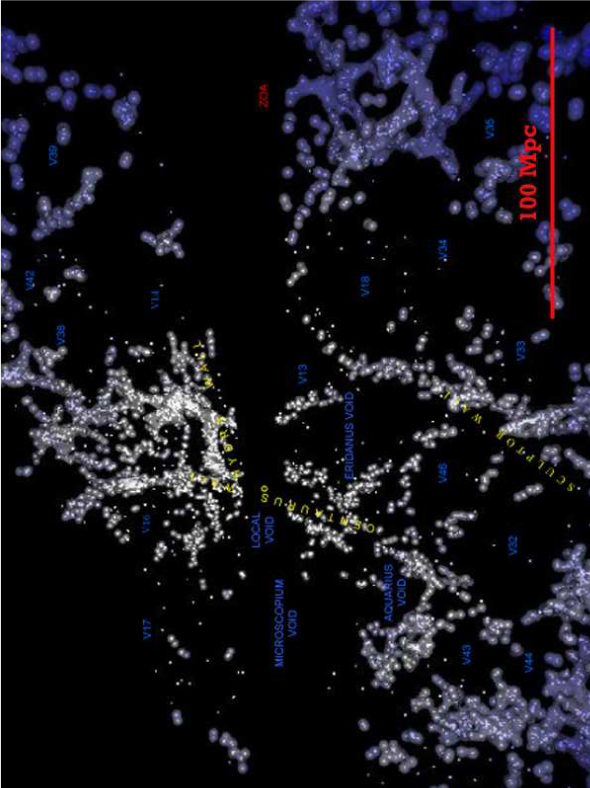
\includegraphics[width=0.32\textwidth, angle =-90]{fairall.png}
  %\includegraphics[width=0.3\textwidth]{fletcher.png}
  \caption{A region of the 6dF redshift survey marked by the presence of various major voids. The image concerns a 3D rendering of the galaxy distribution in a $\SI{1000}{\kilo \metre \per \second}$ thick slice along the supergalactic (SGX) direction, at SGX $= \SI{-2500}{\kilo \metre \per \second}$. Image courtesy of A. Fairall.}
  \label{fig}
\end{center}
\end{figure}
\vspace{-1cm}

\section*{Methods}
\vspace{-0.3cm}
I will start with the introduction to cosmological parameters that help in identifying the voids using existing work by \cite{lindner_structure_1995},  \cite{thompson_historical_2011} and \cite{van_de_weygaert_cosmic_2011}. The Sloan Digital Sky Survey (SDSS) has been the most expansive sky surveying project yet, and this work will extensively discuss several of its aspects, from the processes involved in collecting the data to the conclusions which can be drawn from it. Publicly available catalogs like \cite{pan_cosmic_2012}, \cite{sutter_response_2013} will be used to study the preliminary idea of void galaxy distribution, which will then be discussed extensively through a more recent work \citep{tavasoli_void_2021}. Lastly, the current theories of physical cosmology and how do voids might challenge them will also be addressed.
%I will synthesize research from multiple sources, including a recent textbook on the subject \citep{Shukurov+Subramanian21},
%which contains detailed explanations of magnetic field observations and dynamo theory.
%Moreover, I will make use of a recent review which compiled recent observational data \citep{Beck+19},
%and will refer to the references therein, as needed.
%These sources do not discuss direct numerical simulations in detail, 
%but these have become a crucial tool for understanding magnetic fields.
%Therefore, I will consult some recent literature on this topic \citep[e.g.][]{Pakmor+18,Gent+21}.
%An image of the magnetic field of a spiral galaxy from a zoom-cosmological simulation simulation, 
%along with an observational model is shown in Fig.~\ref{fig}.

\section*{Research output}
\vspace{-0.3cm}
The work will be submitted to \textit{Monthly Notices of the Royal Astronomical Society}. 

\section*{Timeline}
\vspace{-0.3cm}
The work will require 10 weeks in total.
I will spend the first week in learning the basics of distance measures in cosmology, 
followed by two weeks exploring the basics of void observation and identification techniques using the projects like SDSS.
The next two weeks will be spent studying observational and theoretical results from the literature concerning the void galaxy properties and their distribution.
The next two weeks will be devoted to review the consistency of theories of physical cosmology to that of observations and conclusion made from the study of cosmic voids.
The final three weeks will be spent writing the report, while continuing to consult the literature.

\section*{Summary}
\vspace{-0.3cm}
I propose to review the current status of research on cosmic voids and void galaxies
by compiling a fairly exhaustive study, including the most recent findings that can aid in furthering the interest in this field.

%--------------------------------------------------------------------------------------------------------------------------------------------
\bibliographystyle{mnras}
\bibliography{p463}

\end{document}
